\chapter{Cassandra}
\label{appendix:Cassandra}
Cassandra ist eine NoSql Datenbank, die nach dem Wide-Column Model konzipiert ist. Cassandra vereint verschieden Eigenschaften von Googles BigTable \cite{bigtable} und Amazons Dynamo \cite{dynamo}. Sie wurde 2010 von Facebook entwickelt, um das Inbox Search Problem zu lösen \cite{cassandra}. Es ist eine verteilte Datenbank, die sich unter dem CAP-Theorem als AP charakterisieren lässt, wobei man das Level an Konsistenz manuell einstellen kann.

\section{Daten Model}
\label{sec:DM}
Das Daten Modell von Cassandra entspricht dem von BigTable, also dem Wide-Column Modell. Dies beruht im Wesentlichen, wie alle Arten an NoSql Datenbank Modellen auf Key-Value-Stores. Dabei wird für einen Primary Key jeweils eine Reihe mit Column-Families definiert. Die Column-Families bestehen wiederum aus einem Key, der sie beschreibt, und einem Value der dann den Wert angibt. Der Wert kann allerdings wieder eine Menge an Column-Families sein, wodurch es möglich ist Column-Families beliebig zu verschachteln. Es wird bei der Initialisierung angegeben welchen Typ der Wert hat, Verschachtlung wird über benutzerdefinierte Typen erzeugt.
\begin{figure}[htbp!]
	\centering
	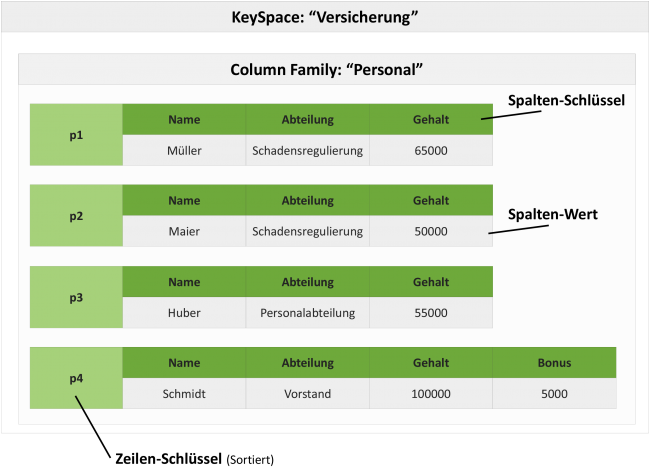
\includegraphics[scale=0.45]{pics/colfam.png}
	\figuresource{http://wi-wiki.de/doku.php?id=bigdata:spaltendb}
	\caption{Beispiel Daten Modell}
	\label{fig:bspDM}

\end{figure} Column-Families, die wiederum Column-Families beinhalten, bezeichnet man als Super-Column-Families. Bei Cassandra werden bei der Initialisierung einer Tabelle, die auch nichts anderes ist als eine Super-Column-Family, alle möglichen Column-Families angegeben. Sie definiert darüber hinaus den Primary Key über den auf die Werte der Column-Families zugegriffen werden können. Im Unterschied zu herkömmlichen SQL Tabellen ist es aber möglich Werte für diese zu unterschlagen, wie in Abbildung \ref{fig:bspDM} für p1 - p3 dargestellt.\\ 
Ein KeySpace stellt die oberste Schicht des Datenmodells da. Für den KeySpace werden bei der Initialisierung eine Replikationsstrategie und eine Anzahl Replikas angegeben, die zu erstellen sind. Diese gelten dann für alle Tabellen, die unter dem KeySpace erstellt werden.

\section{System}
Implementiert ist Cassandra in Java. Darauf aufbauend sind auch die Basis Java Typen verfügbar. Die Daten werden von Cassandra redundant auf verschiedene Instanzen verteilt. Systemnachrichten werden dabei über UDP verschickt, Anwendungsnachrichten, also Nachrichten, die mit den Daten zu tun haben, per TCP um den Verlust von Nachrichten zu vermeiden. Bei den Systemnachrichten ist dies zu verkraften.

\subsection{Partitionierung}
Die Partitionierung orientiert sich an der von Dynamo \cite{dynamo}. Cassandra benutzt genauso wie Dynamo Consistent-Hashing, um Daten auf die verschiedenen Instanzen zu verteilen. Dabei erhalten die verschiedenen Instanzen einen Wert, der sie uniform über einen vordefinierten Wertebereich verteilt, wie in Abbildung \ref{fig:uniformHashing} abgebildet. Consistent-Hashing macht aus dem Wertebereich einen Ring, über den dann die Daten auf die Instanzen wie folgt verteilt werden. Aus einem Datum wird über die Hashfunktion ein Hash-wert berechnet. Das Datum wird dann auf der Instanz abgespeichert, deren Wert auf dem Ring aufsteigend als nächstes kommt. Dieses Verfahren kann zu einer ungleichen Verteilung der Daten auf die Instanzen führen, sodass dadurch die Performance des Systems ineffizient wird. Cassandra löst diese Problem anders als Dynamo dadurch, dass die Werte der Instanzen an die Verteilung der Daten angepasst werden, wie in Abbildung \ref{fig:adaptedHashing} dargestellt. So sind zwar einige Instanzen für einen größeren Wertebereich zuständig, andererseits kommen in diesem größeren Wertebereich weniger Daten vor, sodass die Daten uniform auf die Instanzen verteilt werden. Wird der Datensatz zu groß, skaliert Cassandra, indem eine Instanz im Consistent-Hashing Ring zwischen den Knoten mit den Meisten Daten eingefügt wird. Danach werden die Bereiche wieder so angepasst, dass alle Instanzen ungefähr gleich belastet sind.
\begin{figure}[htbp!]
	\centering
	\begin{subfigure}[c]{0.49\textwidth}
		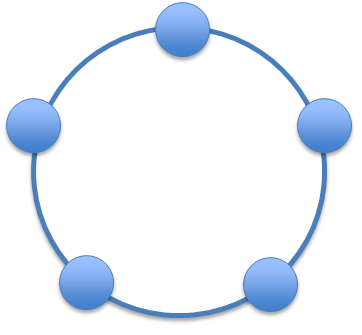
\includegraphics[scale=0.5]{pics/uniformHashing.png}
		\subcaption{Consistent-Hashing uniform distributed instances}
		\label{fig:uniformHashing}
	\end{subfigure}
	\begin{subfigure}[c]{0.49\textwidth}
		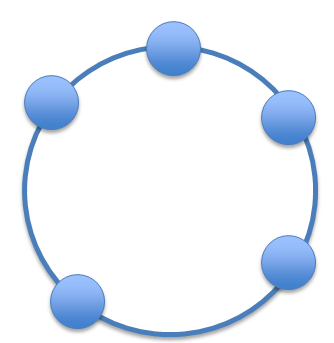
\includegraphics[scale=0.5]{pics/adaptedHashing.png}
		\subcaption{Consistent-Hashing adapted distribution of instances}
		\label{fig:adaptedHashing}
	\end{subfigure}
	\caption{Consistent-Hashing Ring}
\end{figure}

\subsection{Replikation}
Die Art der Replikation in Cassandra ist vom Benutzer konfigurierbar. Die Anzahl der Replikas und die Replikationsstrategie wird durch den KeySpace festgelegt. Dabei kann man zwischen SimpleStrategy und NetworkTopologyStrategy auswählen. Die SimpleStrategy repliziert ohne auf die Netzwerkstruktur einzugehen. Somit beugt sie weniger stark potentiellem Datenverlust vor und sollte daher nur für Test-Zwecke benutzt werden. Sei N die Anzahl Replikas, werden die Daten immer auf die N-1 Nachfolgeknoten repliziert. Bei der NetworkTopologyStrategy wird die Hierarchie von Datacentern und drin enthalten Racs bei der Verteilung betrachtet wird. Somit wird diese Strategie auch für das Deployment empfohlen. Innerhalb dieser Strategie kann man sich wiederum zwischen Rack Aware und Datacenter Aware entscheiden. Dabei werden die Replikas entweder auf verschiedene Racks oder Datacenter verteilt, um die höchst mögliche Datensicherheit zu gewährleisten. Diese Strategien beziehen sich auf den Koordinator, also die Hauptinstanz einer Partition von Daten, da dieser für die Replikation zuständig ist.
Bei der Bestimmung eines Koordinators wird Zookeeper verwendet. Dadurch sind alle Netzwerkänderungen und -konfigurationen persistent gespeichert, da Zookeeper die Konfigurationen jedes Knotens automatisch persistent speichert. Zur Kommunikation werden bei Zookeeper Gossip Algorithmen verwendet.

\subsection{Persistenz}
Persistenz erreicht Cassandra über ein ähnliches System wie BigTable \cite{bigtable}. Zunächst gibt es die MemTable, die im Hauptspeicher gehalten wird und als Cache fungiert. Sie besitzt eine Konfiguration einer Schranke, ab der die MemTable auf die Platte persistiert wird. Auf der Platte gibt es die SSTable, Bloom Filter, index file, compression file und statistics file. Die Daten werden in eine SSTable geschrieben, also eine eigene Datei geschrieben, wenn sie noch nicht vorhanden sind. Wenn dies nicht der Fall ist, wird die betreffende Teil einer SSTable in die MemTable geladen, alle Operationen ausgeführt und die Daten wieder zurück auf die Platte geschrieben. Der Bloom Filter verhindert unnötige Lookups in nicht relevante SSTables. Der Index beschleunigt den Lookup innerhalb einer SSTable. Damit man nicht viele kleine SSTable-Dateien hat werden zwei SSTable, durch einen merge-Prozess immer dann zusammengefasst, wenn eine mindestens halb so groß ist wie die andere. Vorhanden SSTable Files können zusätzlich noch komprimiert werden.

\section{CQL}
Mit CQL (Cassandra Query Language) gibt es eine auf Cassandra zugeschnittene SQL-ähnliche Abfragesprache, die es den Anwendern konventioneller Datenbanken deutlich leichter macht mit Cassandra zu arbeiten. Dabei ist es wichtig zu wissen, dass CQL bei weitem nicht so ausdrucksstark ist wie SQL. Das liegt daran, dass CQL im wesentlich eine abstrakte API für das Cassandra Datenmodell darstellt. In CQL sind normale Datenbank Typen wie int, text, etc. möglich, allerdings kann man auch von Collections wie List, Set und Map Gebrauch machen, da es dafür direkte Java Typen gibt. Des Weiteren ist es möglich eigene Typen zu definieren, wie schon in Abschnitt \ref{sec:DM} beschrieben.\\
\begin{figure}[htbp!]
	\centering
	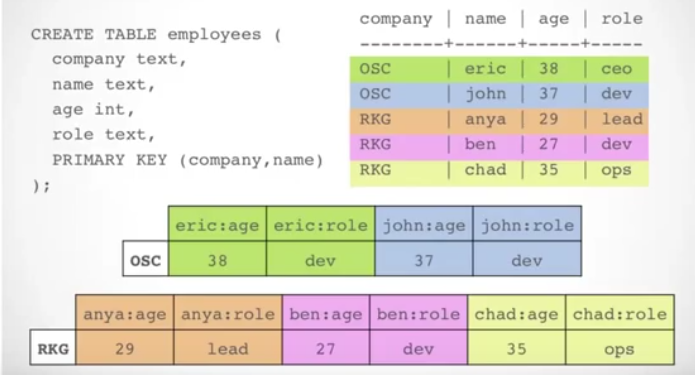
\includegraphics[scale=0.7]{pics/cql_mapping.png}\\
	\figuresource{\url{https://www.youtube.com/watch?v=UP74jC1kM3w}}
	\caption{CQL Mapping}
	\label{fig:mapping}
\end{figure}
Tabellen und Spalten werden wie ebenso in Abschnitt \ref{sec:DM} beschrieben durch Column-Families dargestellt. und wie in SQL erzeugt. Dabei wird ein Primary Key benötigt der dann als Row Key fungiert. Es kann nur über diesen Row Key auf die Zeilen zugegriffen werden. Deshalb kann man in der WHERE-Klausel in CQL auch nur Elemente des Primary Key angeben. Auf diesen Elementen wird durch die Indizierung schon beim Speichern in Cassandra eine Sortierung berechnet was die Anfragen deutlich perfomanter macht. Für alle anderen Spalten der Zeile wäre dies also nicht performant und wird von CQL nicht gestattet. Die Spalten und Zeilen werden wie folgt auf das Cassandra Datenmodell abgebildet.\\
Der erste Teil des Primary Keys bildet, wie man sehen kann, den Row Key, die restlichen Teile werden mit ihren Werten in die Beschreibung der Column-Families integriert, so wie im unteren Teil in Abbildung \ref{fig:mapping} beschrieben. Somit werden alle Zeilen mit dem gleichen ersten Teil des Primary Keys in der gleichen Zeile abgespeichert. Über dieses Mapping ist es möglich eine tabellenartige Abstraktion zu erzeugen, die sich durch CQL ausdrückt und Anwendern ein aus SQL bekanntes Interface bietet.
